\chapter{Discussion}
\label{chp:5_discussion}
%\subsection{Dataset and Model} 

\subsection{Analysis of Failure Cases}
Experimental results show that there are two main restrictions of the proposed method: out of gamut values in the chrominance channels emerging during optimization leading to visible artifacts and failing to generate adversarial images when the original image has limited colorfulness.

\textbf{Out of Gamut Values}: Modifying the chrominance channels in \(YC_{b}C_{r}\) and CIELAB spaces may lead to improper values on individual RGB channels. This is also common in widely used chroma subsampling and mitigating this issue is an open research topic~\cite{chan2008toward}. In our work, we clip the reconstructed RGB to the valid range and feed the target network with the clipped image at each iteration to prevent further change in the pixel values out of the gamut. Clipping also zeroes out the gradient and prevents further updates in gradient based optimization. However, we found that it still causes visible artifacts in the adversarial image, especially around the borders between red and gray tones. Figure~\ref{fig:outofgamut} shows two examples where spatial transformation in red-gray borders yield out of gamut pixels and clipping the values still causes visible artifacts since clipping in RGB space effectively changes the values of luminance channels.

\textbf{Failed Attacks on Less Colorful Images}: Results in Table~\ref{table:foolingrate}, show that the attack success rate does not reach 100\% when spatial transform attack is restricted to chrominance channels.  %We investigated the images that our method fails to fool the network for both \(C_{b}C_{r}\) and \(a^{*}b^{*}\) settings.  
This implies that the chrominance based attacks fail for a number of images in the dataset. Examples of such images are provided in Figure~\ref{fig:fails}. We observed that these  particular images are either monochromatic examples or have a uniform color pattern, for which spatial transformation in a neighborhood lead to little change.
%only having regions where a spatial flow in colorspace would change the pixel values, such as black-color or white-color borders. It can be seen that these images have low colorfulness .
% shows examples from failure cases where our method is not able to generate successful adversarial examples for both colorspaces we used.

To analyze the effect of colorfulness on the attack performance, we calculated the colorfulness index histogram of the images in the dataset (Figure \ref{fig:hist}) . We found that 3.2\% of the dataset consists of grayscale images, for which our method would not be able to make any changes to the input image, inevitably resulting in a failed attack. Figure \ref{fig:plots} shows the attack success rate using the subsets where colorfulness is lower-limited by filtering out examples having colorfulness index less than the \(x\) axis value. Although a*b* attacks are slightly more successful than \(C_bC_r\) in the low colorfulness regime \((<=0.2)\), they have the same success rate of the attacks over higher colorfulness.

%This shows there are still cases our method would not be able to produce successful examples. 

\begin{figure}[t]

    \begin{center}
        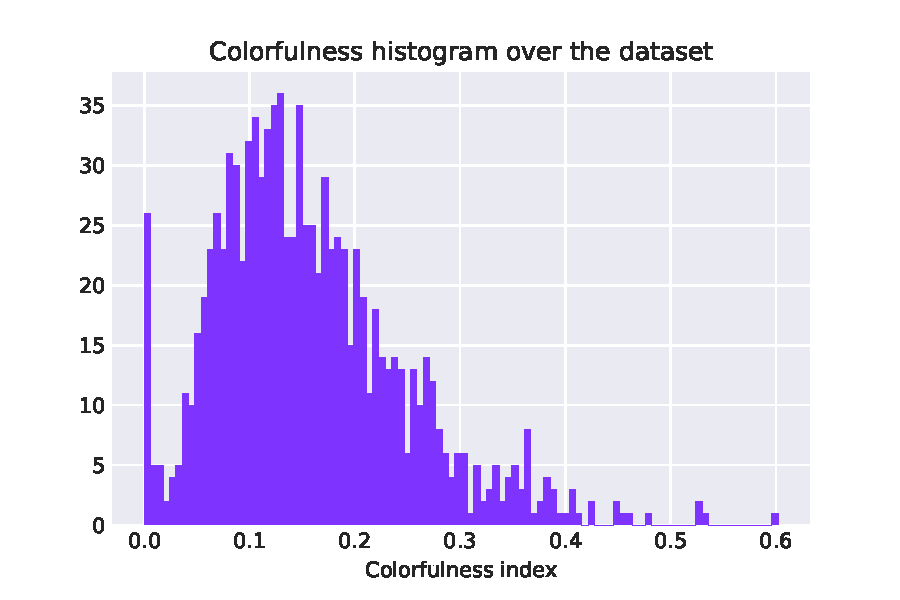
\includegraphics[width=0.92\linewidth]{plots/color_hist.pdf}
    \end{center}
    \caption{Colorfulness index histogram over NIPS2017 dataset.}\label{fig:hist}
\end{figure}
\begin{figure}[t]
    \begin{center}
        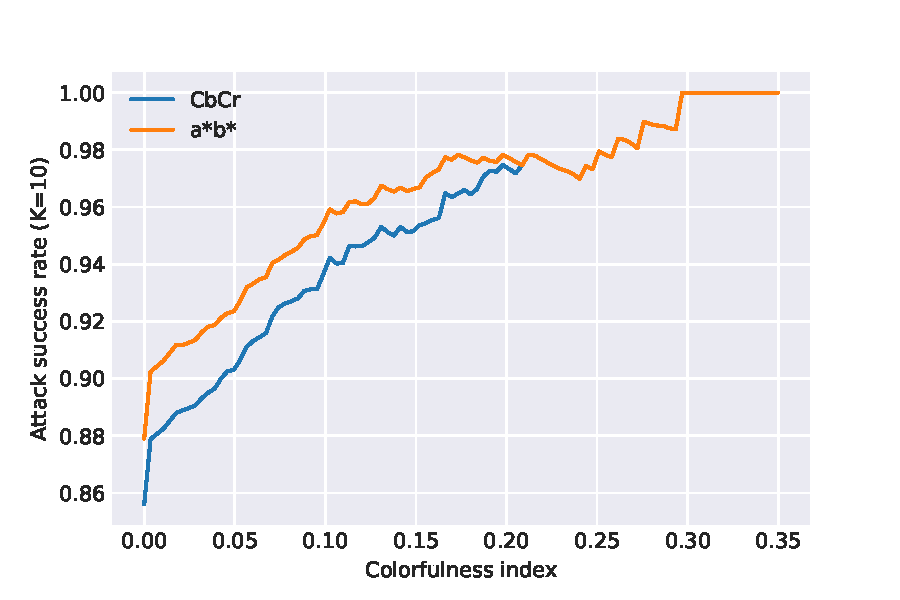
\includegraphics[width=0.92\linewidth]{plots/color_success.pdf}
    \end{center}
    \caption{Attack success rate analysis with regards to colorfulness index with \(\kappa=10\) on \(CbCr\) and a*b* channels. Images having colorfulness index less than the \(x\) axis value are excluded in calculation of the success rate. Note that both colorspaces attain very close success rates after around colorfulness index 0.2.} \label{fig:plots}
\end{figure}

%We find that 32 images in the dataset are in grayscale.

\begin{figure}[t]
    %burasi neden boyle cikiyor henuz cozemedim
    % \includegraphics[width=0.30\linewidth]{fails/1.png}
    % \includegraphics[width=0.30\linewidth]{fails/2.png}
    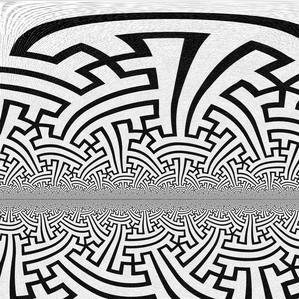
\includegraphics[width=0.328\linewidth]{fails/3.png}
    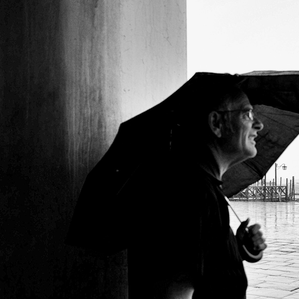
\includegraphics[width=0.328\linewidth]{fails/7.png}
    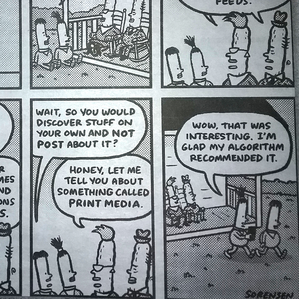
\includegraphics[width=0.328\linewidth]{fails/8.png}
    % 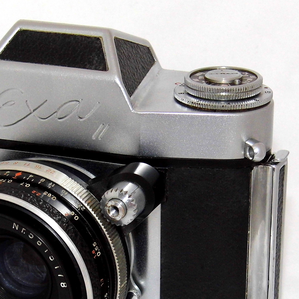
\includegraphics[width=0.328\linewidth]{fails/10.png}
    % 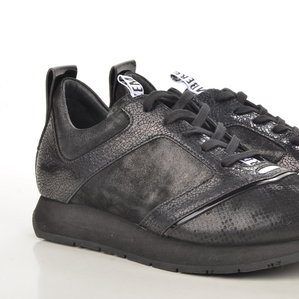
\includegraphics[width=0.328\linewidth]{fails/11.png}
    % 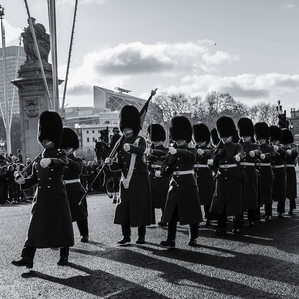
\includegraphics[width=0.328\linewidth]{fails/12.png}
    % 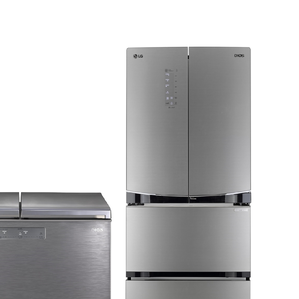
\includegraphics[width=0.328\linewidth]{fails/15.png}
    % 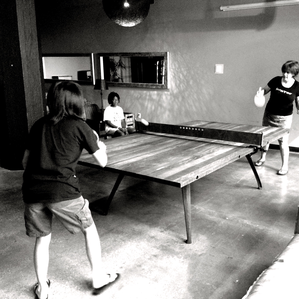
\includegraphics[width=0.328\linewidth]{fails/17.png}
    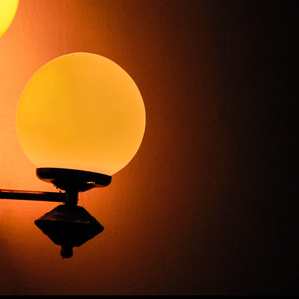
\includegraphics[width=0.328\linewidth]{fails/6.png}
    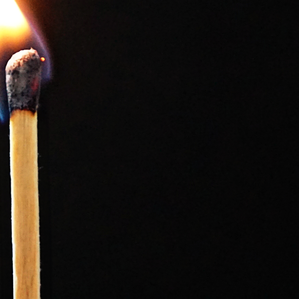
\includegraphics[width=0.328\linewidth]{fails/13.png}
    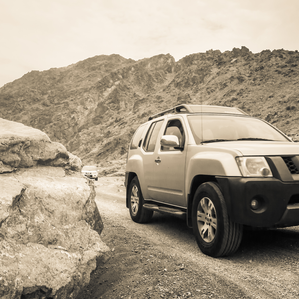
\includegraphics[width=0.328\linewidth]{fails/5.png}
    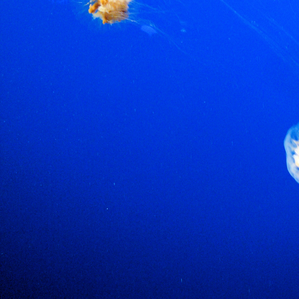
\includegraphics[width=0.328\linewidth]{fails/9.png}
    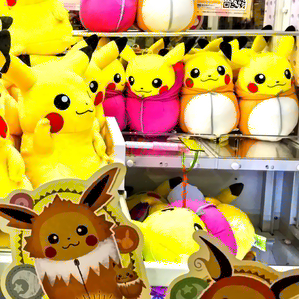
\includegraphics[width=0.328\linewidth]{fails/4.png}
    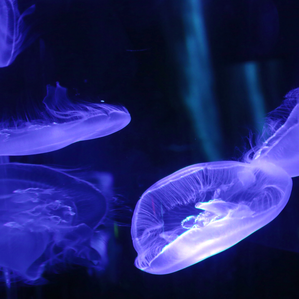
\includegraphics[width=0.328\linewidth]{fails/14.png}
    \caption{Examples from the dataset that our method fails to generate successful adversarial examples from in both \(YC_{b}C_{r}\) and CIELAB spaces, sorted from top bottom by colorfulness amount.}\label{fig:fails}
\end{figure}


\begin{figure}[H]
    %burasi neden boyle cikiyor henuz cozemedim
    \includegraphics[width=0.495\linewidth]{outofgamut/1.png}
    \includegraphics[width=0.495\linewidth]{outofgamut/2.png}
    \caption{Examples of visible clipping artifacts of out-of-gamut pixels caused by spatial transform around red-gray borders. Flow magnitude has been scaled up to highlight the visible effects for illustration.}\label{fig:outofgamut}
\end{figure}


\section{Discussion}\label{section:discussion}
As it can be seen by Figure~\ref{fig:fails}, the input images that our method fails are generally grayscale or monochromatic images, which prevents chrominance spatial transforms from changing the pixel values due to the low magnitude of chrominance channel values. In addition, input images having a very limited local color variation negatively affect the performance by limiting the potential search space. We observed that there is a significant drop in the success rate with the setup confidence margin \(\kappa=10\) if the attack is restricted to subpixel changes in comparison to the unrestricted attacks. We argue that this performance drop is arising from the fact that the most examples are already JPEG compressed, which means chroma subsampling is applied to the benign examples, which restricts the subpixel restricted search space by dramatically reducing the local chrominance variation. This leads to the observation that chroma subsampling could be an effective defense method against our attack. Moreover, the search space is further restricted in JPEG compressed images as the quantization step of JPEG compression attenuates high frequency information, especially in the chrominance channels. Nonetheless, we observed adversarial examples generated by spatial transforms in chrominance channels of perceptual colorspaces obtain competitive fooling rates without making perceptible changes to the image. This observation provides further evidence for the hypothesis that representation of deep neural networks does not necessarily align with human vision ~\cite{geirhos2018imagenet}.

